\section{Task 4, 5 and 6 - Flag Game}
\subsection{The task}
The game consists of guessing the capitals of three random flags from a given pool.

The user writes the number on the input text near each flag. This number is taken from the shown list of capital cities. All fields must be filled in to submit a guess.

If the answers are correct, it increases the user points by three, otherwise it decreases them by one. It then returns to the main page.
\subsection{Game page}
\subsubsection{game.jsp}
At the start of the page we create a Capitals object: this objects has two fields, \textit{capitals} and \textit{chosen\_capitals}, which are both String arrays. At the object creation, the constructor fills \textit{capitals} with city names and shuffle it, then it chooses three random and add them to \textit{chosen\_capitals}.

We also get the user with the same method from \textit{Main.java}, so that we can be redirected if we do not have an authentication.

In the page, we show the same header as the main page, then an ordered list that shows \textit{capitals} and a form with an entry for each element of \textit{chosen\_capitals}. This form has for each label an image and an input field. The image is saved in the system as \textit{(capital\_name).png}, so it is easy to get it from the chosen capital value. The input field is of type number, required and has value \textit{min=0} and \textit{max=(capitals.lenght())}. The name value is taken from a Capitals method \textit{findCapitalId()}, which takes as an input a city name and returns its index in \textit{capitals}. This way, the url that gets the form results has only to compare the field name and field value.
\subsubsection{Game.java}
The GET method simply redirects to the \textit{game.jsp} page.

The POST method, as sad before, compares the field names and values to determine if the user got all responses correctly. It then updated the user session and the context (as asked for task 8) and redirects to the main page.


\subsubsection{Screenshots}
\begin{figure}[H]
  \centering
  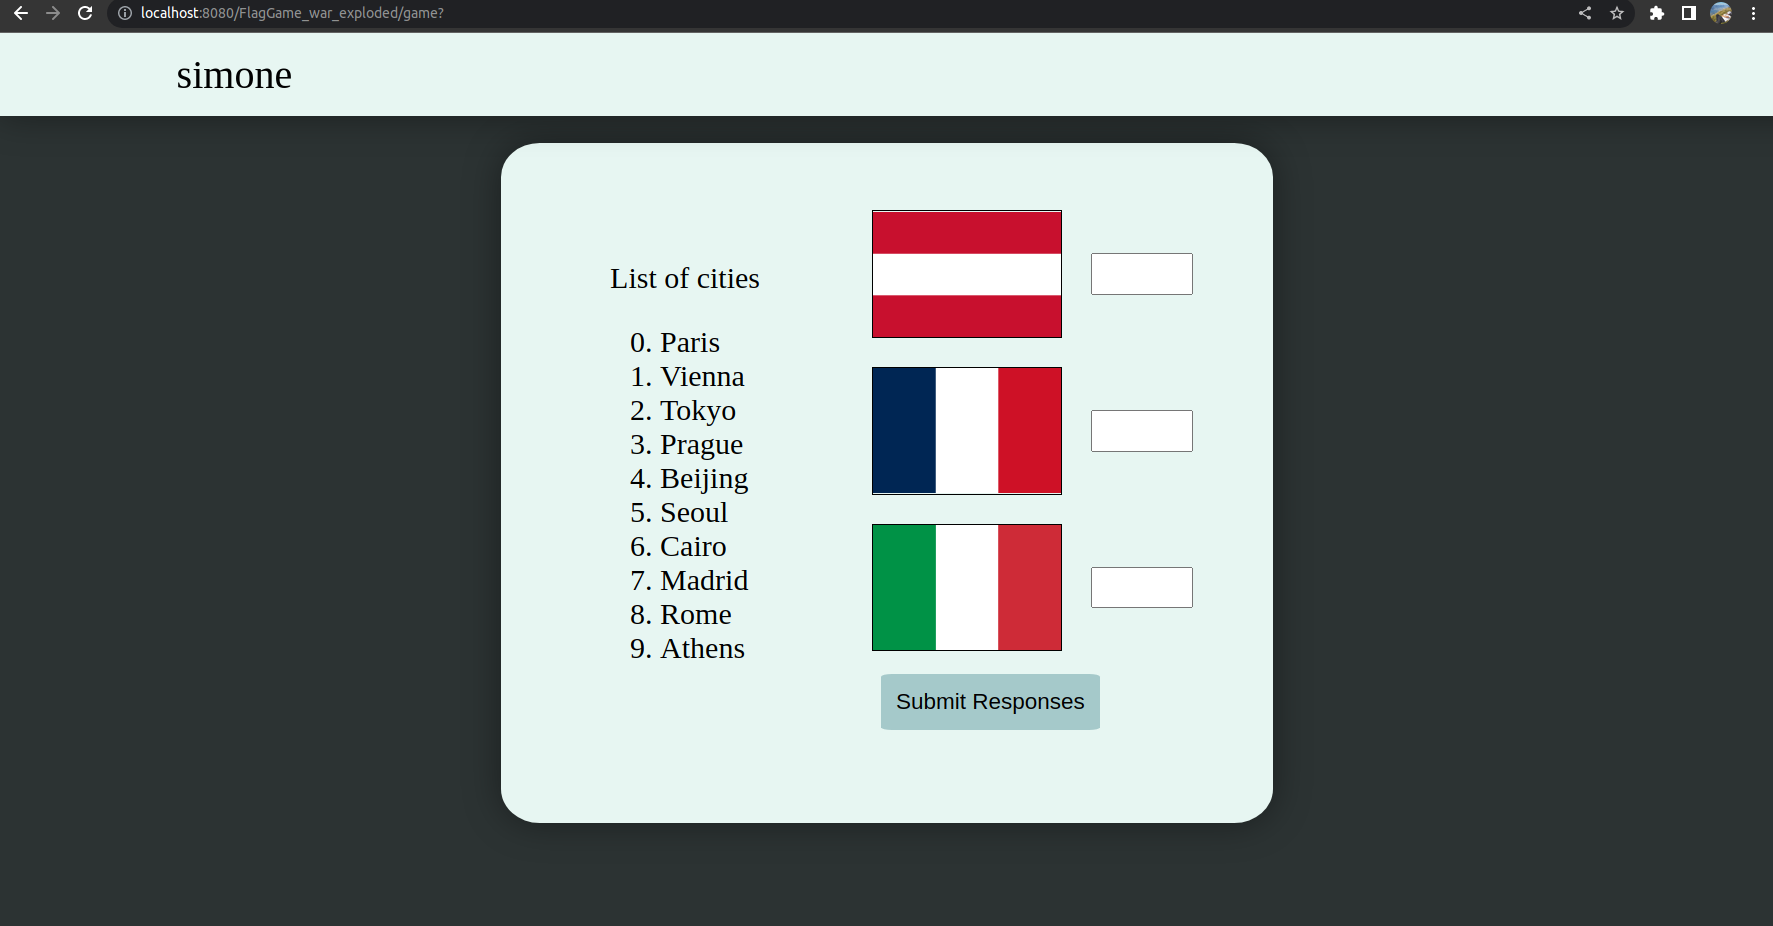
\includegraphics[width=\columnwidth]{game_1.png}
  \caption{Flag Game}
\end{figure}
\begin{figure}[H]
  \centering
  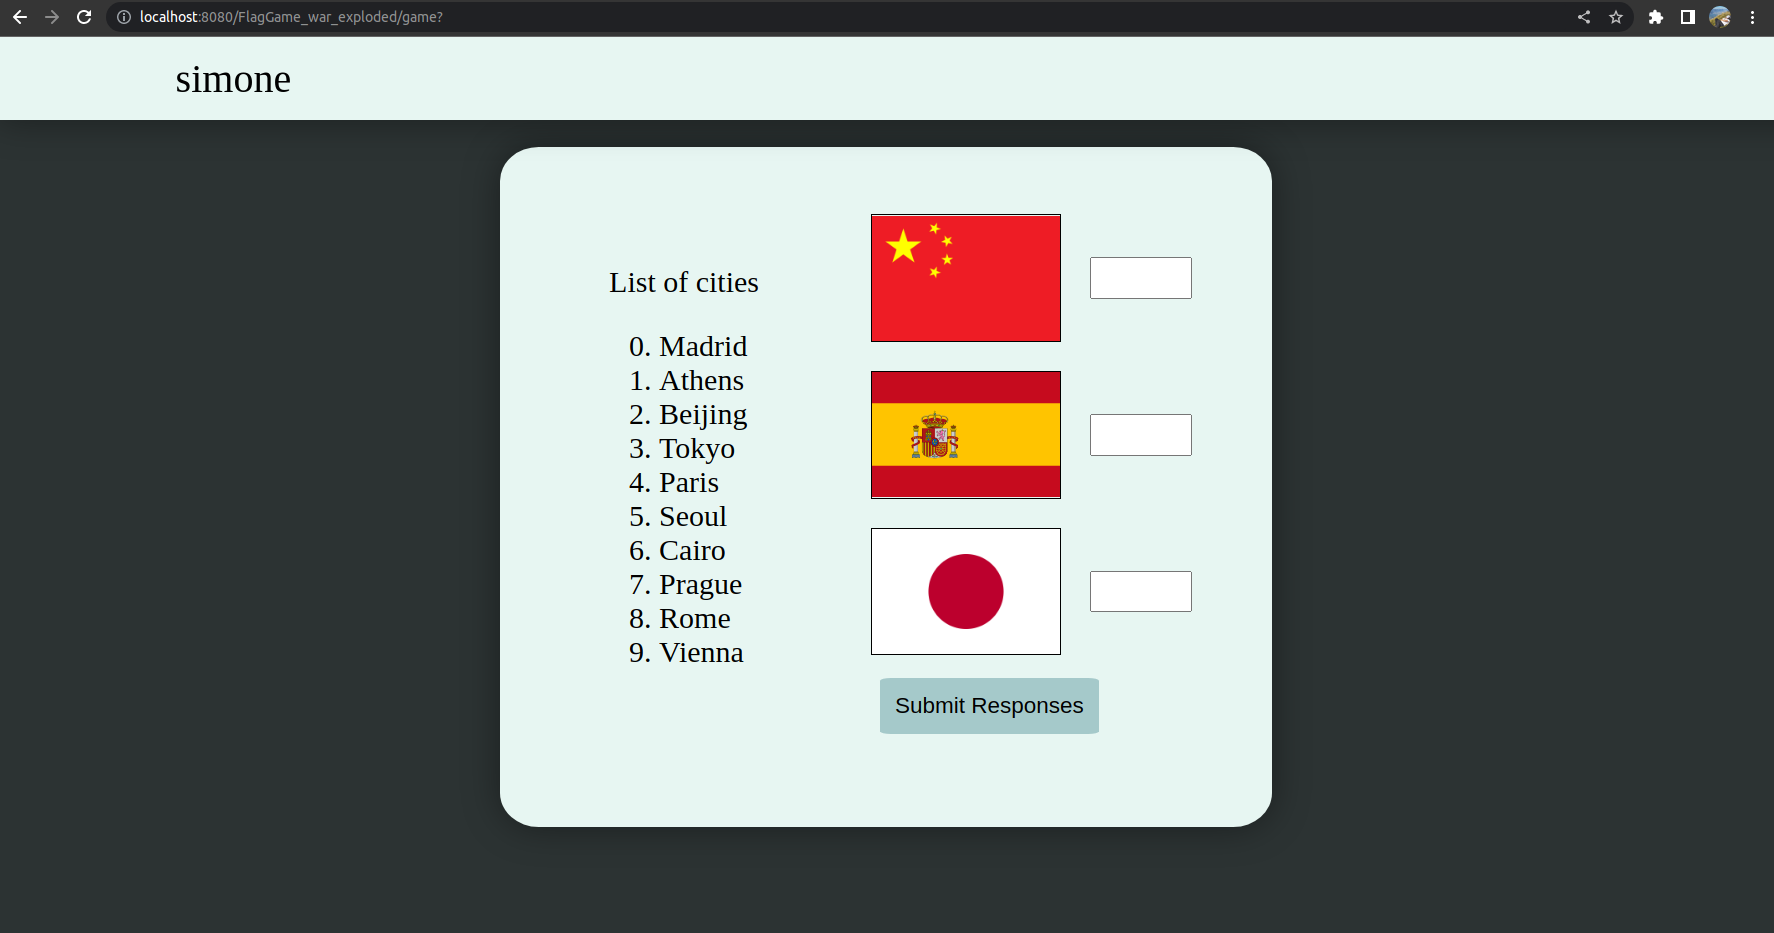
\includegraphics[width=\columnwidth]{game_2.png}
  \caption{Flag Game, another example}
\end{figure}